\documentclass[11pt]{article}

% Packages kept to a standard set so this compiles on Overleaf and on a basic TeX install.
\usepackage[a4paper,margin=1in]{geometry}
\usepackage[T1]{fontenc}
\usepackage{lmodern}
\usepackage{microtype}
\usepackage{amsmath,amssymb,amsthm}
\usepackage{graphicx}
\usepackage{booktabs}
\usepackage{caption}
\usepackage{float}
\usepackage{xcolor}
\usepackage[numbers,sort&compress]{natbib}
\usepackage[colorlinks=true,linkcolor=blue!50!black,citecolor=blue!50!black,urlcolor=blue!50!black]{hyperref}

\graphicspath{{figures/}}
\captionsetup{font=small,labelfont=bf}

\newtheorem{claim}{Claim}
\newtheorem{conjecture}{Conjecture}
\newtheorem{lemma}{Lemma}
\theoremstyle{remark}
\newtheorem*{remark}{Remark}

\newcommand{\kap}{\kappa}
\newcommand{\Wmax}{W^{\max}}
\newcommand{\Wmin}{W^{\min}}
% TODO (Kevin): replace with the GitHub URL once the remote exists.
\newcommand{\repourl}{\textcolor{red}{\texttt{[GitHub link to be added]}}}

\title{\textbf{Kingmakers and Formats:}\\[2pt]
How Much of Who Wins Is Decided by the Tournament When Matchups Are Cyclic?}
\author{Kevin Kinsey S (EP23B027) \quad and \quad Aditri Jain (ED23B060)\\[2pt]
\small DA5453: Learning from Human Preferences, IIT Madras \\
\small Project report on Chen \& Joachims,\\ \small\emph{Modeling Intransitivity in Matchup and Comparison Data} (WSDM 2016)}
\date{27 November 2026}

\begin{document}
\maketitle

\begin{abstract}
\noindent
Bradley--Terry (BT) gives every player one strength number, so it cannot express rock--paper--scissors matchups. Blade--Chest
(BC) can. Chen and Joachims show that BC \emph{predicts} better on cyclic data, but not whether this changes any decision made
with the model. We study one such decision: running a knockout tournament. We split every matchup table into a ladder part and
a cycle part, define the cyclic share $\kap\in[0,1]$, and measure exactly, over all 315 brackets of 8 players, how many
players an organiser can make the favourite ($K$) and how far they can move a player's title chance ($\Pi$). Under BT the
organiser can already crown several of the top players, but never the weakest one; this follows from a 1978 theorem that we
re-derive. As $\kap$ grows, both $K$ and $\Pi$ rise steadily (medium-decisive matches: $K$ from 2.0 to 7.9, $\Pi$ from 0.09 to
0.20), and the weakest player becomes crownable only when cycles dominate. Fitting BT to cyclic data hides about two-thirds of
this power, while BC recovers it and is preferred on held-out matches. In ATP tennis, held-out data show no usable cycles. Finally,
round robin's edge over a knockout in crowning a ``deserving'' winner disappears as $\kap\to 1$.
\end{abstract}

% ============================================================================================================
\section{Question, why it matters, and approach}
\label{sec:intro}

\subsection{From the paper to our question}
In this course we presented Chen and Joachims' Blade--Chest paper~\cite{chen2016blade}. Its starting point is simple. The
standard model of who-beats-whom, Bradley--Terry~\cite{bradley1952rank} (the model behind Elo ratings~\cite{elo1978rating}),
gives each player one number $g_i$ and says $i$ beats $j$ with probability $\sigma(g_i-g_j)$. One number per player means
the players sit on a \emph{ladder}: if A usually beats B and B usually beats C, then A must beat C. Real games do not always
work like that. In a strategy game, an aggressive style can beat a defensive one, which beats a greedy one, which beats the
aggressive one. Blade--Chest gives each player two extra vectors, a ``blade'' (how they attack) and a ``chest'' (how they
defend), so that matchups can go round in circles. The paper's evidence is predictive: on professional StarCraft~II the
blade--chest model improves test accuracy by about 5\%, while on tennis and DotA~2 it barely beats Bradley--Terry.

After presenting it, we kept returning to a question the paper does not ask: \emph{so what?} A better log-likelihood is
nice, but nobody runs a tournament on log-likelihood. Pairwise models are used to \emph{make decisions}: to seed brackets, to
rank chatbots from human votes (Chatbot Arena fits Bradley--Terry to pairwise human preferences~\cite{chiang2024arena}), and
to train the reward models behind RLHF~\cite{ouyang2022training}. Human preferences are themselves known to be intransitive
at times~\cite{tversky1969intransitivity}. If the world has cycles and the model does not, are those decisions wrong, and
by how much?

We picked the most visible decision of this kind: a \textbf{knockout tournament}. It is also where the paper's own data come
from: its StarCraft matches were played in single-elimination, double-elimination, group and round-robin events, many with a
random draw~\cite[\S4.3.1]{chen2016blade}. Most of us have heard someone say a player ``only won because of the draw''. Under a
ladder, the draw can only shuffle luck around, because the best player is the best against everyone. Under cycles, the
draw decides \emph{who meets their counter}. Figure~\ref{fig:p4} (Section~\ref{sec:theory}) shows a 4-player example in which
the player with the lowest average win rate is the favourite, purely because of the bracket.

\subsection{The question}
\begin{quote}
\emph{When matchups are cyclic, how much of who wins is decided by the tournament (its bracket and its format) rather than by
the players? We measure this as a function of how cyclic the matchups are, with Bradley--Terry and Blade--Chest as the two
models of the world.}
\end{quote}
This breaks into three concrete questions.
\begin{enumerate}
\item[\textbf{Q1}] \textbf{Bracket power.} How many players can an organiser make the favourite by choosing the bracket, and
which ones? Does that change from a ladder to a cycle?
\item[\textbf{Q2}] \textbf{Model choice.} If we estimate the matchups from data with BT or with BC, do we see the same organiser
power? Which estimate should we believe?
\item[\textbf{Q3}] \textbf{Formats.} If cycles make the bracket matter, do fairer formats (round robin, Swiss, groups) fix it, and
at what cost in matches?
\end{enumerate}

\subsection{Why it is worth asking}
\begin{itemize}
\item \textbf{Fairness has a hidden parameter.} If the bracket can change the champion, the organiser is a kingmaker. Whether
that power is small or large depends on how cyclic the matchups are, which nobody usually measures.
\item \textbf{It turns a modelling choice into a consequence.} BT versus BC stops being a question of a few points of
log-likelihood and becomes ``does the model even see that the tournament can be rigged?''
\item \textbf{It tests where Bradley--Terry's assumption actually matters.} Classic results say that under BT stronger players
do better in any slot of a bracket~\cite{chung1978stronger}. We can ask what breaks when that assumption is dropped, which is
exactly the kind of ``remove an assumption and find the counterexample'' question a theory project can answer.
\end{itemize}

\subsection{Key idea and approach}
\textbf{One dial for cyclicity.} Any matchup table can be split exactly into a ladder part and a cycle part (the Hodge
decomposition on the complete graph~\cite{jiang2011hodge}). The cyclic share $\kap\in[0,1]$ is the fraction of the table
that is cycle. $\kap=0$ is a pure Bradley--Terry ladder and $\kap=1$ is pure rock--paper--scissors. We generate matchups at
any $\kap$ we like, and we also estimate $\kap$ from data.

\textbf{Measure organiser power exactly.} For 8 players there are only 315 genuinely different brackets, and a short dynamic
program gives every player's exact title chance in each one. So we do not estimate the organiser's power; we compute it:
\begin{itemize}
\item $K$ = the number of players who are the unique favourite of \emph{some} bracket (the ``crownable'' players);
\item $\Pi$ = the average, over players, of the best-bracket minus worst-bracket title chance (the ``swing'').
\end{itemize}
Around this core we run (i) numerical counterexample searches before any proof, with exact arithmetic for every example we
quote; (ii) BT and BC fits to sampled match data from a synthetic strategy game and to ATP tennis; (iii) a check of what
standard Elo seeding promises versus what it delivers; and (iv) simulations of five tournament formats.
Figure~\ref{fig:setup} summarises the pipeline.

\begin{figure}[!htbp]
\centering
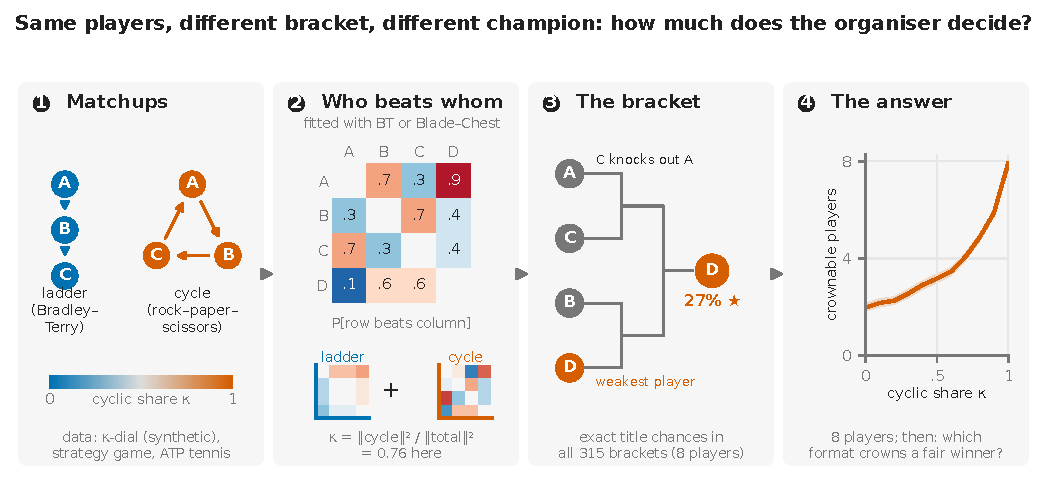
\includegraphics[width=\textwidth]{F0_setup.pdf}
\caption{Setup. (1) Matchups range from a ladder to a cycle; we generate them at a chosen cyclic share $\kap$ or estimate them
from data. (2) A matchup table $P$ is split into ladder and cycle parts; the example is the 4-player table of
Figure~\ref{fig:p4}. (3) For a table $P$ we compute every player's exact title chance in every bracket. (4) We summarise how much
the bracket decides (here, the number of crownable players versus $\kap$, from Section~\ref{sec:e1}) and compare formats.}
\label{fig:setup}
\end{figure}

\subsection{What we found}
\begin{enumerate}
\item \textbf{A ladder can already be rigged at the top, but it protects the bottom.} Under BT a non-best player can be made the
favourite (up to $n-1$ of the $n$ players), but the weakest player never can. This follows from Chung and Hwang's
theorem~\cite{chung1978stronger}, which we re-derived before finding it. In every BT table we tested, the crownable players
form a block at the top of the ranking (a new conjecture).
\item \textbf{Cycles hand the organiser more power, gradually.} With 8 players and medium-decisive matches, $K$ rises from
about 2 at $\kap=0$ to 3.5 at $\kap=0.6$ and about 8 at $\kap=1$, and $\Pi$ roughly doubles. The weakest player becomes
crownable only once cycles dominate ($\kap\gtrsim 0.6$--$0.8$). Rigging needs \emph{both} decisive matches and cycles.
\item \textbf{You see this power only if your model can see cycles, and only if the cycles are real.} On a synthetic strategy
game, a BT fit underestimates organiser power about threefold; BC recovers it and predicts held-out matches better in 20 of 20
instances. On ATP tennis, held-out data show no usable cycles, and an over-fitted BC model would invent them.
\item \textbf{Formats.} Round robin's advantage over a 7-match knockout in crowning a ``deserving'' winner shrinks to zero as
$\kap\to1$. In a mostly-ladder world an Elo-seeded knockout gets most of round robin's benefit with a quarter of the matches;
in a mostly-cyclic world extra matches buy almost nothing.
\end{enumerate}

% ============================================================================================================
\section{Background: models, the cyclic share, and the bracket computation}
\label{sec:background}

\paragraph{Matchups.} There are $n$ players ($n=4$ and $8$ for exact work, $16$ for search). $P_{ij}$ is the probability that
$i$ beats $j$, with $P_{ij}+P_{ji}=1$. The logits $L=\operatorname{logit}(P)$ form a skew-symmetric matrix.

\paragraph{Bradley--Terry and Blade--Chest.} BT sets $L_{ij}=g_i-g_j$. The blade--chest inner-product model
\cite[eq.~4]{chen2016blade} sets
\begin{equation}
L_{ij} = g_i - g_j + b_i\!\cdot c_j - b_j\!\cdot c_i, \qquad b_i, c_i\in\mathbb{R}^d,
\end{equation}
where $b_i$ is player $i$'s blade and $c_i$ their chest. The extra term is skew-symmetric and can create cycles: with $d=2$
and three players whose blades and chests point $120^\circ$ apart, it reproduces rock--paper--scissors. The paper regularises
with $\lambda\sum_i\|b_i-c_i\|^2$.

\paragraph{The cyclic share $\kap$.} For any skew-symmetric $L$, let $s_i = \frac1n\sum_j L_{ij}$ (a player's \emph{strength
score}) and split
\begin{equation}
L = T + C,\qquad T_{ij}=s_i-s_j\ \text{(ladder part)},\qquad C = L-T\ \text{(cycle part)}.
\end{equation}
Every row of $C$ sums to zero, $T$ and $C$ are orthogonal in the Frobenius inner product, and $T$ is the least-squares BT fit
to $L$. This is the Hodge decomposition on the complete graph~\cite{jiang2011hodge}. We define
\begin{equation}
\kap = \frac{\|C\|_F^2}{\|L\|_F^2}\in[0,1].
\end{equation}
Throughout, ``weakest player'' means the lowest strength score $s_i$. (Under cycles there is no canonical weakest player; we
also recorded the lowest average win rate, with similar conclusions.)

\paragraph{Generating matchups at a chosen $\kap$.} We draw a random ladder $\hat T$ (from $g\sim N(0,I)$) and a random cycle
$\hat C$ (a random skew-symmetric matrix with its ladder part removed), both normalised to unit norm, and set
\begin{equation}
L = \text{scale}\cdot\big(\sqrt{1-\kap}\,\hat T + \sqrt{\kap}\,\hat C\big),\qquad P=\sigma(L).
\end{equation}
Because $\hat T\perp\hat C$, the realised cyclic share is exactly $\kap$ (checked to $10^{-15}$). We also use structured
cycles built from random $d=2$ blade--chest vectors (``BC-d2''). The \emph{scale} sets how decisive matches are. We use
three scales, calibrated so that at $\kap=0$ a typical match (mean $|P_{ij}-\tfrac12|$) is 58--42 (``close''), 68--32
(``medium'') or 82--18 (``decisive''). The calibration barely drifts with $\kap$: at $\kap=1$ the means are 0.078, 0.176
and 0.311 instead of 0.08, 0.18 and 0.32.

\paragraph{Brackets and exact title chances.} A bracket places the $n$ players on the leaves of a balanced binary tree.
Swapping the two halves under any node gives the same tournament, so there are $n!/2^{n-1}$ distinct brackets: 3 for
$n=4$, 315 for $n=8$, and 638{,}512{,}875 for $n=16$. For a node $v$ with child subtrees $A$ and $B$, the probability that
$i\in A$ comes out of $v$ is
\begin{equation}
q_v(i) = q_A(i)\sum_{j\in B} q_B(j)\,P_{ij},\qquad q_{\text{leaf}}=1,
\end{equation}
and player $i$'s title chance is $W_i(\sigma)=q_{\text{root}}(i)$. This costs $O(n^2)$ per bracket, so all 315 brackets of 8
players take milliseconds.

\paragraph{Measuring organiser power.} For each player, $\Wmax_i=\max_\sigma W_i(\sigma)$ and $\Wmin_i=\min_\sigma W_i(\sigma)$,
and the \emph{swing} is $R_i=\Wmax_i-\Wmin_i$. A player is \emph{crownable} if some bracket makes them the unique favourite
(ties within $10^{-12}$ do not count). Then
\[
K(P)=\#\{\text{crownable players}\},\qquad \Pi(P)=\frac1n\sum_i R_i .
\]
\emph{A small example.} Take the BT strengths $g=(1.0,\,0.95,\,0.8,\,-3.0)$ for A, B, C, D: three nearly equal players and one
hopeless one. The three brackets give:
\begin{center}
\small
\begin{tabular}{lccccc}
\toprule
Bracket & $W_A$ & $W_B$ & $W_C$ & $W_D$ & Favourite \\
\midrule
\{A,B\} $|$ \{C,D\} & 0.287 & 0.267 & \textbf{0.446} & 0.000 & C (3rd strongest) \\
\{A,C\} $|$ \{B,D\} & 0.287 & \textbf{0.500} & 0.213 & 0.000 & B (2nd strongest) \\
\{A,D\} $|$ \{B,C\} & \textbf{0.520} & 0.267 & 0.213 & 0.000 & A (strongest) \\
\bottomrule
\end{tabular}
\end{center}
Whoever is drawn against D gets a near-free pass to the final, and that is worth more than a small skill gap. So $K=3$ (every
player except D), and A, B and C each have a swing of 23.4 points, giving $\Pi\approx0.175$. Note that even this pure ladder
can be rigged: the organiser can make the 3rd-best player the favourite. (Values computed exactly in
\texttt{theory/verify\_examples.py}.)

\paragraph{Formats.} For $n=8$ we compare five formats (match counts in parentheses): a knockout with a uniformly random bracket
(KO-random, 7); a knockout seeded by a BT ranking with the standard 1v8, 4v5, 2v7, 3v6 pattern (KO-elo, 7); a 3-round Swiss
system (12); two round-robin groups of four followed by semi-finals and a final (Groups+KO, 15); and a full round robin (28).
To judge whether a format crowns a ``deserving'' winner we use three references, because under cycles there may be no best
player: the Copeland winner(s) (most head-to-head wins), the Borda winner (highest average win probability), and the Nash
mass $x$ of the zero-sum game with payoff $P-\tfrac12$ (Nash averaging~\cite{balduzzi2018reevaluating}).

% ============================================================================================================
\section{Theory: what a ladder guarantees, and how cycles break it}
\label{sec:theory}

Our rule was \emph{numerical falsification first, proof second}: run an aggressive counterexample search, and only then
try to prove a claim. All code is in \texttt{theory/}.

\paragraph{Deterministic outcomes (P1, cited).} If every match is certain and the results form a ladder, the top player wins
every bracket and $K=1$. If certain results contain cycles, deciding whether a given player can win some bracket is the
tournament-fixing problem: Vassilevska Williams~\cite{williams2010fixing} shows that a ``king'' who beats at least half the
field can be made to win under suitable conditions, with refinements in~\cite{kim2015fixing,manurangsi2022fixing}. (With
certain outcomes a champion must win $\log_2 n$ matches, so at $n=4$ a player with only one win can never be crowned, cycles or
not.) Our interest is the probabilistic case in between, where every player can win any match with some probability.

\subsection{Under Bradley--Terry, stronger players do better in any slot}
\begin{claim}[P3; Chung and Hwang~\cite{chung1978stronger}]
Under BT, let $g_i>g_j$. Take any bracket $\sigma$, and let $\sigma'$ be $\sigma$ with $i$ and $j$ exchanged. Then
$W_i(\sigma')>W_j(\sigma)$: put the stronger player in the weaker player's slot and they do strictly better than the weaker
player did there.
\end{claim}
We first found this numerically: 0 violations in 999{,}480 random tests at $n=4$, 8 and 16, plus 2.4 million evaluations of an
adversarial hill-climb that tried to break it. The same detector flags violations immediately on cyclic tables, so the zero
is meaningful. We then proved it, and only afterwards found that it is the main theorem of Chung and Hwang (1978), who prove
it for every tree shape and every $n$. We cite it as theirs. Our route is independent and short for $n=4$; we include it
because it shows exactly where the BT assumption is used.

\begin{proof}[Proof for $n=4$]
Write $a_u=e^{g_u}$, so $P(u\text{ beats }v)=a_u/(a_u+a_v)$. The BT property we use is
\begin{equation}
\label{eq:star}
g_i>g_j \;\Rightarrow\; P(i\text{ beats }m) > P(j\text{ beats }m)\ \text{for every other player } m. \tag{$\star$}
\end{equation}
\emph{Case 1: $i$ and $j$ meet in round one.} Then $\sigma'=\sigma$, and each player's title chance is ``win the semi''
times ``beat the other semi's winner''. Since $P_{ij}>P_{ji}$ and, by~\eqref{eq:star}, $i$ beats every possible finalist more
often than $j$ does, $W_i>W_j$.

\emph{Case 2: they are in different semis.} Call the other two players $x$ and $y$, and let $\sigma$ be
\{$i$ vs $x$\} $|$ \{$j$ vs $y$\}, so $\sigma'$ is \{$j$ vs $x$\} $|$ \{$i$ vs $y$\}. Then
\[
W_j(\sigma) = P_{jy}\,\big[P_{ix}P_{ji}+P_{xi}P_{jx}\big],\qquad W_i(\sigma') = P_{iy}\,\big[P_{jx}P_{ij}+P_{xj}P_{ix}\big].
\]
The first factor is ``win the semi against $y$'', and $P_{iy}>P_{jy}$ by~\eqref{eq:star}. The bracket is ``beat the survivor
of the other semi'', where the other semi is the swapped player against $x$. Writing $u,v,w$ for the odds $a_i,a_j,a_x$ and clearing the
positive denominators $(u+v)(v+w)(u+w)$, their difference is
\[
u^2(v+w)+2uvw - v^2(u+w) - 2uvw = (u-v)(uv+uw+vw) > 0 .
\]
So both factors are larger for $i$, and $W_i(\sigma')>W_j(\sigma)$.
\end{proof}
For larger brackets the same factorisation reduces the claim to a ``ladder lemma'' about a player climbing past $h$
opponents in turn. We verified that lemma symbolically for $h\le4$ (all brackets up to 32 players): the difference
always factors as $(u-v)$ times a polynomial with only positive coefficients. Chung and Hwang's induction covers all $h$.

\paragraph{Consequences.}
\begin{itemize}
\item \textbf{The weakest player is never the favourite} (any $n$). Take $i$ to be the weakest player's first-round opponent,
who is stronger; exchanging first-round opponents leaves the bracket unchanged, so Case 1 gives $W_i>W_{\text{weakest}}$.
\item \textbf{Up to $n-1$ players can be crowned, and this is tight.} With $n-1$ nearly equal players and one hopeless one,
whoever is drawn against the hopeless player is the favourite. We found $K=7$ of 8 numerically.
\item \textbf{A player's title chance rises with their own strength}, with everything else fixed (also Adler et
al.~\cite{adler2017random}).
\end{itemize}

\begin{conjecture}[P6, new]
Under BT the crownable players always form a top block: if the $r$-th strongest is crownable, so are the $1$st to
$(r-1)$-th.
\end{conjecture}
We noticed this in the experiments of Section~\ref{sec:e1}: it holds in all 1{,}200 BT tables there, and in 230{,}000 random
and 615{,}000 adversarial tests at $n=4$ and $8$. It does not follow directly from P3, because after swapping $i$ into $j$'s
slot a third player might overtake $i$. With cycles it fails quickly: the crownable set is a top block in 98.7\% of tables
at $\kap=0.1$ but only 87.8\% at $\kap=0.6$. So a ladder lets the organiser choose among the top players but never reach
down the table.

\subsection{Cycles break it: the weakest player can be the favourite}
Chung and Hwang note that their theorem needs more than ``stronger players beat weaker ones'' (strong stochastic transitivity),
and Israel~\cite{israel1981stronger} later showed that even the averaged version fails without BT. Cycles break it in the most
visible way possible. Figure~\ref{fig:p4} shows a 4-player table with one-decimal probabilities. D has the lowest average win
rate (0.43) and the lowest strength score, yet in the bracket \{A vs C\} $|$ \{B vs D\} D is the favourite, with
\[
W_D = P_{DB}\,\big(P_{AC}P_{DA}+P_{CA}P_{DC}\big) = 0.6\,(0.3\cdot0.1+0.7\cdot0.6) = 0.27 \quad\text{exactly},
\]
ahead of C (0.252), A (0.246) and B (0.232). D's only bad matchup is A, and A's nemesis C knocks A out 70\% of the time.
Under BT this is impossible: if C beats A and A beats D 90\% of the time, BT forces C to beat D far more than 40\% of the time.
The table has $\kap=0.76$.

\begin{figure}[!htbp]
\centering
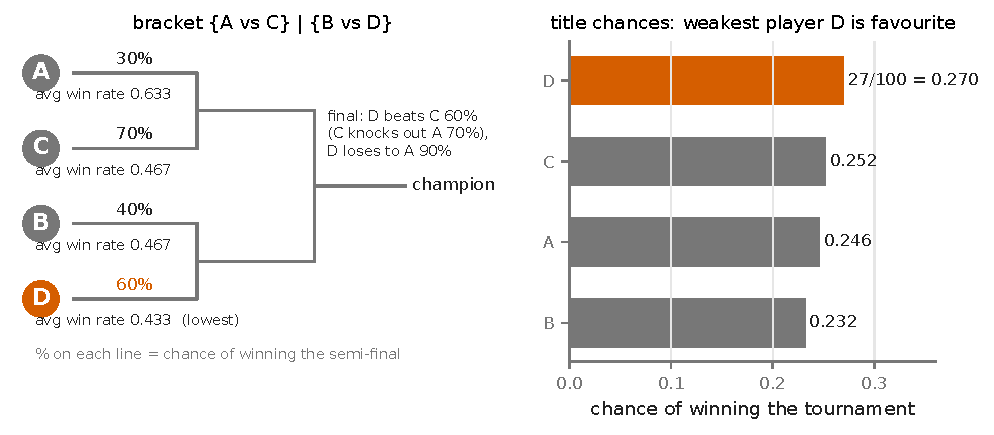
\includegraphics[width=\textwidth]{F1_p4_example.pdf}
\caption{Cycles let the weakest player be crowned (P4). Left: the bracket \{A vs C\} $|$ \{B vs D\}, with each player's average
win rate and chance of winning the semi-final; the full table is in Figure~\ref{fig:setup}(2). Right: exact title chances. D,
who has the lowest average win rate, is the favourite at exactly $27/100$.}
\label{fig:p4}
\end{figure}

\paragraph{How much cyclicity does it take?} Over all 531{,}441 tables with probabilities in $\{0.1,\dots,0.9\}$, the weakest
player can be crowned in 1{,}584, and the smallest $\kap$ among them is 0.755. A continuous search over tables with all
probabilities in $[0.05,0.95]$ found an example at $\kap=0.56$, and none lower. This is evidence, not a proven threshold. It
already suggests the pattern that Section~\ref{sec:e1} confirms at 8 players: crowning the very bottom player needs cycles to
dominate.

% ============================================================================================================
\section{Experimental setup}
\label{sec:setup}

\paragraph{Synthetic matchups.} 8 players; $\kap\in\{0,0.1,\dots,1\}$; three decisiveness scales; random-skew and BC-d2
cycles; 200 random tables per setting, each analysed over all 315 brackets. For 16 players we cannot enumerate 638 million
brackets, so we use local search (swap two players, keep improvements, 10 random restarts). Validated at 8 players, it hits
the exact optimum 98\% of the time, so the 16-player numbers are lower bounds on $\Wmax$ and on $K$.

\paragraph{A synthetic strategy game.} To get data that look like a real cyclic game, we built a purely synthetic ``archetype
game''. Three play styles counter each other in a loop, with blade and chest directions $120^\circ$ apart in $d=2$. Each player
is one style plus individual noise (s.d.\ 0.3) plus their own skill $g\sim N(0,0.5^2)$, with cycle strength 0.8. These values
were fixed \emph{before} any organiser-power metric was examined, to hit $\kap\approx0.6$; the 20 instances used have
$\kap=0.63\pm0.03$. From each true table we sample $N\in\{10,50\}$ matches per pair, plus separate validation and test
matches, and fit BT (maximum likelihood) and BC ($d=2$, the paper's regulariser, $\lambda$ chosen on validation log-loss).

\paragraph{Real data: ATP tennis.} We used Jeff Sackmann's \texttt{tennis\_atp} match files for 2015--2019~\cite{sackmann2024tennis}
and took the 16 players with the most matches against each other (614 matches: Djokovic, Federer, Nadal, Murray, and others).
We split them by time: the first 80\% for fitting and $\lambda$ selection, the last 20\% for testing.

\paragraph{Reproducibility.} Every experiment script takes \texttt{--quick}/\texttt{--full} and writes a CSV whose header
records the seed, parameters, git commit and runtime. Every number in this report comes from one of those CSVs. The full
pipeline runs in about 10 minutes on a laptop, and 41 unit tests and 26 sanity checks (Appendix~\ref{app:sanity}) pass. Code:
\repourl.

% ============================================================================================================
\section{Results: organiser power}
\label{sec:results}

\subsection{Organiser power grows with the cyclic share}
\label{sec:e1}
\begin{figure}[!htbp]
\centering
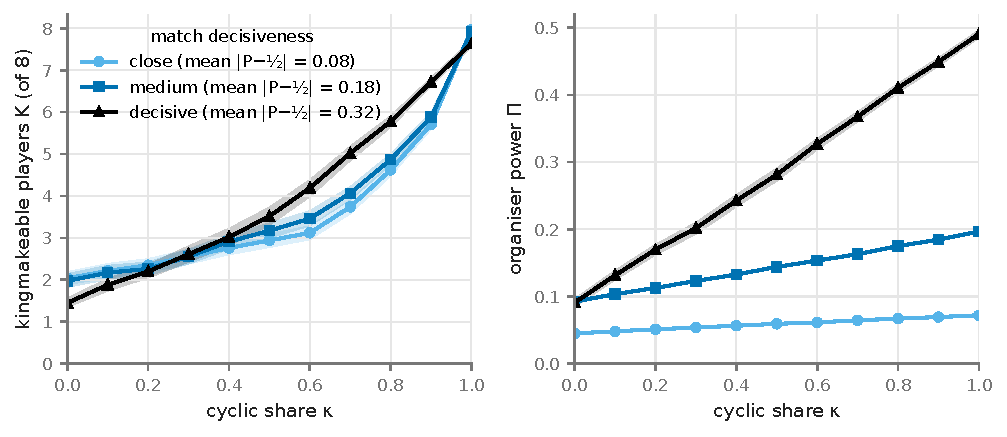
\includegraphics[width=\textwidth]{F2_power_vs_kappa_skew.pdf}
\caption{Organiser power versus cyclic share (8 players, all 315 brackets, 200 tables per point, random-skew cycles; shading is
a 95\% bootstrap CI). Left: number of crownable players $K$. Right: average swing $\Pi$. Lines are the three decisiveness
levels, labelled by the mean distance of a match probability from a coin flip at $\kap=0$.}
\label{fig:e1}
\end{figure}

Figure~\ref{fig:e1} is the headline result. Table~\ref{tab:e1} gives the numbers.
\begin{table}[!htbp]
\centering\small
\begin{tabular}{lcccccc}
\toprule
& \multicolumn{3}{c}{crownable players $K$ (of 8)} & \multicolumn{3}{c}{average swing $\Pi$} \\
\cmidrule(lr){2-4}\cmidrule(lr){5-7}
scale & $\kap=0$ & $\kap=0.6$ & $\kap=1$ & $\kap=0$ & $\kap=0.6$ & $\kap=1$ \\
\midrule
close    & 2.04 [1.89, 2.20] & 3.12 [2.96, 3.29] & 7.97 & 0.045 & 0.061 & 0.072 \\
medium   & 1.98 [1.82, 2.15] & 3.46 [3.29, 3.65] & 7.93 & 0.092 & 0.153 & 0.197 \\
decisive & 1.45 [1.34, 1.57] & 4.19 [3.98, 4.39] & 7.64 & 0.091 & 0.327 & 0.490 \\
\bottomrule
\end{tabular}
\caption{Organiser power, random-skew cycles (mean and 95\% CI). CIs on $\Pi$ are narrower than $\pm0.003$. BC-d2 cycles give
nearly the same values (medium: $K$ = 1.94, 3.45, 7.74).}
\label{tab:e1}
\end{table}

\begin{itemize}
\item \textbf{Both measures rise steadily with $\kap$}, at every scale and for both kinds of cycle. Mean $K$ increases in 59 of
60 adjacent steps of $\kap$ (the exception is within the CIs).
\item \textbf{The bottom of the table is reached last.} The weakest player is crownable in 0 of 200 tables in every setting
with $\kap\le0.5$. At $\kap=0.9$ it is crownable in 3\% (close), 13\% (medium) and 43\% (decisive) of tables. Crownability
spreads \emph{down} the ranking gradually: at medium scale, the lowest-ranked crownable player goes from rank 2.0 at $\kap=0$
to 3.5 at $\kap=0.6$ and 8 at $\kap=1$.
\item \textbf{Rigging needs two ingredients.} We expected more decisive matches to mean \emph{less} organiser power, since a
dominant player cannot be dethroned. That is true in a ladder: at $\kap=0$, decisive matches give the \emph{fewest} crownable
players (1.45), and $\Pi$ stops growing with decisiveness (0.092 at medium, 0.091 at decisive). In a cycle it reverses: no
player is safe from a counter, and decisiveness only amplifies the organiser's choice of who meets whom ($\Pi$ = 0.07, 0.20,
0.49). Close matches remove the first ingredient (bracket choices matter little when every match is near a coin flip); a
ladder removes the second.
\item \textbf{The trend holds at 16 players} (local search, 20 tables per point, medium scale; lower bounds): $K\ge4.9$ at
$\kap=0$, $\ge9.5$ at $0.6$ and 16 at 1; $\Pi\ge0.106$, 0.158, 0.204.
\end{itemize}
We checked these numbers independently with a separate pure-Python script, written from the definitions, that enumerates all
40{,}320 seedings without using our bracket code. It reproduces $K$ exactly on 96 of 96 tables and $\Pi$ to $3\times10^{-17}$.

\subsection{Fitting the wrong model hides the organiser's power}
\label{sec:e2}
In practice we never see $P$; we see match results and fit a model. Here we ask whether BT and BC, fitted to the same
sampled matches, see the same organiser power. To estimate the swing we fit a model, treat its fitted table as true, and run
the same 315-bracket computation.

\begin{table}[!htbp]
\centering\small
\begin{tabular}{llcccc}
\toprule
matches per pair & table & held-out log-loss & $\kap$ & $K$ & $\Pi$ \\
\midrule
--- & true $P$ & 0.563 & 0.65 & $4.20\pm0.37$ & $0.197\pm0.009$ \\
10 & BT fit & $0.665\pm0.005$ & 0 & $2.15\pm0.27$ & $0.066\pm0.004$ \\
10 & BC fit & $0.607\pm0.010$ & 0.59 & $4.10\pm0.35$ & $0.199\pm0.013$ \\
50 & BT fit & $0.656\pm0.004$ & 0 & $2.30\pm0.26$ & $0.063\pm0.004$ \\
50 & BC fit & $0.575\pm0.005$ & 0.65 & $4.50\pm0.27$ & $0.199\pm0.009$ \\
\bottomrule
\end{tabular}
\caption{Archetype game, 8 players, 20 instances (mean $\pm$ s.e.). Lower log-loss is better.}
\label{tab:e2}
\end{table}

\begin{figure}[!htbp]
\centering
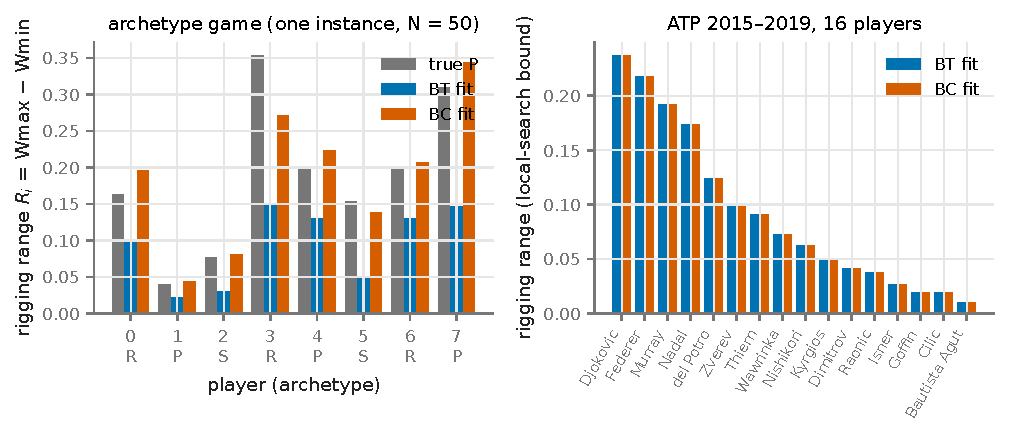
\includegraphics[width=\textwidth]{F3_rigging_bt_vs_bc.pdf}
\caption{Per-player swing $R_i$ (best minus worst bracket). Left: one archetype-game instance (50 matches per pair); letters give
each player's style. The BT fit flattens every player's swing; the BC fit tracks the truth. Right: ATP tennis 2015--2019, where
BT and BC fits coincide (both lower bounds from local search over 16-player brackets).}
\label{fig:e2}
\end{figure}

\textbf{BT underestimates organiser power about threefold} (Table~\ref{tab:e2}): $\Pi=0.063$ against a true 0.197, and it misses
about half the crownable players. The reason is that BT is fitted with no cycle part, so it irons the counters out of the
table. Its answer is correct for the world it describes, which is the wrong world. \textbf{BC recovers both} ($\Pi=0.199$,
$K=4.5$), and \textbf{held-out matches say which to believe}: BC has lower test log-loss in 20 of 20 instances at 50 matches per
pair (by $0.081\pm0.006$ nats per match) and in 19 of 20 at 10 per pair. With only 10 matches per pair, BC gets the average
power right, but its \emph{set} of crownable players overlaps the true set less well (Jaccard 0.64 versus 0.79 at 50).

\paragraph{Tennis looks like a ladder.} On the 614 ATP matches, BT and BC have the same held-out log-loss (0.6416 and
0.6415; a coin flip scores 0.6931). Validation selects a $\lambda$ large enough to shrink BC all the way to BT, so the fitted
$\kap$ is 0. The organiser can still crown a top block of at least four players (Djokovic, Federer, Nadal, Murray; $\Pi\ge0.092$),
as P6 predicts. This agrees with Chen and Joachims, who also found little gain over BT on tennis. Two explanations seem
plausible to us, though we have not tested them: the 16 players are pre-selected elite players whose games are close to
complete, and a single set of rules on a court may average styles out more than a strategy game with explicit counters does.

\paragraph{An over-fitted cyclic model invents cycles.} With weak regularisation, BC ``finds'' $\kap\approx0.7$--$0.8$ in the
tennis data and fits the training matches much better (log-loss 0.495 versus 0.589), but it is far worse on later matches
(1.13--1.81). So \textbf{$\kap$ must be estimated out of sample}, or organiser power will be overstated.

\subsection{Seeding by a ranking in a cyclic world}
\label{sec:e3}
Real organisers do not choose brackets to rig them. They rank the players (Elo, ATP points), then seed by rank: 1st plays 8th
in round one, 4th plays 5th, 2nd plays 7th, 3rd plays 6th, and the top two seeds are placed in opposite halves so they can
only meet in the final. That ranking is a BT ladder. So we ask: for an \emph{honest} organiser using standard seeding, how far
are the ranking's promised title chances from the real ones when the world has cycles?

For each table we fit BT, build the seeded bracket, and compute every player's title chance twice: as the BT ranking predicts
(``promised'') and under the true table (``actual'').

\begin{figure}[!htbp]
\centering
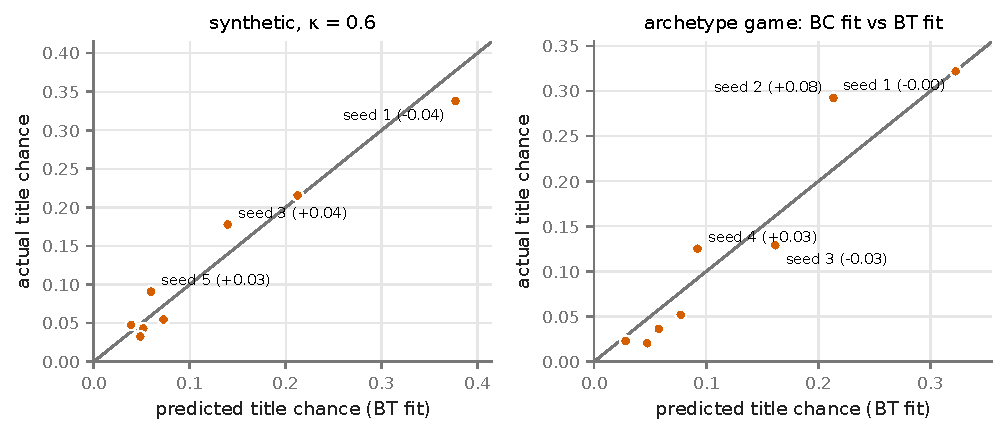
\includegraphics[width=\textwidth]{F4_elo_pred_vs_actual.pdf}
\caption{Promised (BT ranking) versus actual title chance in the Elo-seeded bracket, one example table each. Left: synthetic,
$\kap=0.6$. Right: archetype game (actual = BC fit). Points on the diagonal are promises kept; points above it are luckier than
promised. Labels show the top seed and the three largest misses, with the gain in brackets.}
\label{fig:e3}
\end{figure}

\begin{itemize}
\item \textbf{With no cycles the promises are exact} (control, $\kap=0$: difference $<10^{-16}$).
\item \textbf{With cycles they drift.} In each table, the largest miss averages 4.6 points at $\kap=0.3$, 6.9 at $\kap=0.6$, and
9.2 in the archetype game (between the BT and BC fits), with individual misses up to 22 points (Figure~\ref{fig:e3}).
\item \textbf{The top seed is protected less than promised.} Under a ladder, the seeded bracket is better for the top seed than
87\% of all 315 brackets. At $\kap=0.6$ that falls to 65\%, and the top seed's actual title chance is 1.7 points below the
promise on average. The reason: seeding hands the top seed the \emph{overall} weakest opponents, but ``weakest overall'' is not
the same as ``easy for me''; the 8th seed may be exactly the top seed's counter.
\item \textbf{Gains and losses follow styles, not rank}: a seed whose path avoids their counter-style gains, and one whose path
runs into it loses. A one-number ranking cannot see this.
\end{itemize}
So even without any intent to rig, ladder-based seeding in a cyclic world hands out hidden advantages.

% ============================================================================================================
\section{Results: which format crowns a sensible winner?}
\label{sec:formats}

\begin{figure}[!htbp]
\centering
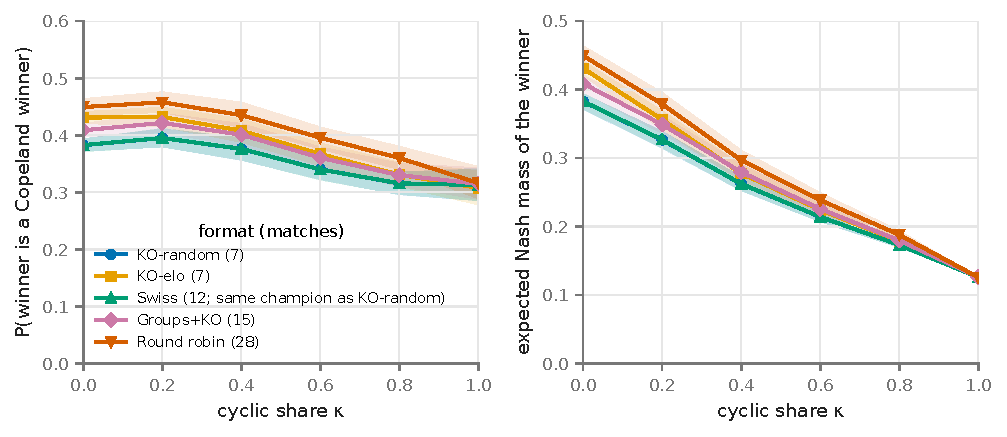
\includegraphics[width=\textwidth]{F5_formats_vs_kappa.pdf}
\caption{Five formats (8 players, medium scale, 200 tables per point; matches played in brackets). Left: probability that the
winner is a Copeland winner. Right: expected Nash mass of the winner. Swiss coincides with KO-random (see text).}
\label{fig:e4}
\end{figure}

We simulated each format 10{,}000 times per table (exact computation for the knockouts) at $\kap\in\{0,0.2,\dots,1\}$.
Figure~\ref{fig:e4} shows the results, and Table~\ref{tab:e4} gives each format's gain over a random knockout on the same tables.
\begin{table}[!htbp]
\centering\small
\begin{tabular}{lccc}
\toprule
format (matches) & $\kap=0$ & $\kap=0.6$ & $\kap=1$ \\
\midrule
Round robin (28 matches) & $+0.067$ [0.063, 0.070] & $+0.055$ [0.052, 0.059] & $+0.003$ [0.002, 0.005] \\
KO-elo (7)               & $+0.048$ [0.046, 0.050] & $+0.027$ [0.019, 0.034] & $-0.005$ [$-0.014$, 0.004] \\
Groups+KO (15)           & $+0.026$ [0.025, 0.027] & $+0.020$ [0.019, 0.022] & $+0.002$ [0.001, 0.003] \\
Swiss (12)               & $0.000$ & $0.000$ & $0.000$ \\
\bottomrule
\end{tabular}
\caption{Gain in the probability that the winner is a Copeland winner: paired difference from KO-random on the same
tables (95\% bootstrap CI). The Nash-mass gains shrink faster: round robin's falls from
$+0.067$ at $\kap=0$ to $+0.024$ at $0.6$ and 0 at 1.}
\label{tab:e4}
\end{table}

\paragraph{Mostly-ladder worlds ($\kap\lesssim0.4$).} Round robin is the most reliable, crowning a Copeland winner about 6--7
points more often than a random knockout. But an Elo-seeded knockout gets about 70\% of that gain with 7 matches instead of
28. Groups+KO uses 15 matches and gains less than the seeded knockout. If matchups are close to a ladder, a seeded
knockout is the efficient choice and round robin is the thorough one.

\paragraph{Mostly-cyclic worlds ($\kap\gtrsim0.8$).} The advantage of seeding disappears first (it relies on the ranking
being right), and by $\kap=1$ all five formats coincide, on a winner distribution that is nearly uniform (entropy 2.9--3.0
bits; uniform over 8 players is 3 bits). Extra matches buy almost nothing, because there is no clear deserving winner to find:
Copeland, Borda and Nash disagree, and the Nash strategy spreads over about 7 of the 8 players. What remains is the organiser's
power over the bracket (Section~\ref{sec:e1}). In that regime, a transparent random draw is the defensible choice: it does no
worse than seeding and cannot be steered.

Round robin's advantage shrinks as $\kap$ grows on all three references, and reaches zero at $\kap=1$. A reversal appears
only for Borda at $\kap=1$ and is 0.2 points, which is negligible.

\paragraph{A side observation about Swiss.} With 8 players and 3 rounds of ``most wins'', the Swiss system crowns
\emph{exactly} like a random knockout. Round 2 pairs the four 1--0 players at random, and round 3 forces the two 2--0 players to
meet, so the champion's path is a random bracket; the 5 extra matches only sort out the lower places. Our simulations agree with
the exact random-knockout values within Monte Carlo error.

% ============================================================================================================
\section{Discussion}
\label{sec:discussion}

\paragraph{Is ``the best player'' even defined under cycles?} Under a ladder, all three references (Copeland, Borda, Nash)
pick the same player. As $\kap$ grows they separate, and at $\kap=1$ the Nash strategy spreads over almost everyone. So the
honest answer to ``which format crowns the best player'' becomes ``there is no best player to crown''. A format can only
choose \emph{which} notion of deserving it rewards, and the bracket then chooses among the candidates.

\paragraph{Is rigging power a flaw or unavoidable?} Under a ladder, the organiser can choose only among the top players, and
the weakest is protected by a theorem. Under cycles every bracket favours someone, because every bracket decides who meets
their counter. The power is a property of the matchups, not a defect of knockout tournaments. A random draw does not remove
it; it only takes the choice away from the organiser. That is why we recommend a random draw for cyclic games.

\paragraph{Does the BT-versus-BC choice change the verdict?} Yes, and in a predictable direction. A BT fit always reports a
ladder, so it always reports a ladder-sized organiser power, about a third of the truth in our cyclic game. BC reports
cycles only when held-out data support them: it matched the true power in the game and collapsed to BT on tennis.

\paragraph{A note on the paper's regulariser.} Chen and Joachims regularise with $\lambda\sum_i\|b_i-c_i\|^2$. We found that
this restrains the \emph{size} of the vectors only weakly: as $\lambda$ goes from 0.01 to 1000, the fitted blades lengthen
(mean norm 2 to 36) without changing $\kap$, and the fit collapses to BT only near $\lambda=10^5$. With our first grid capped at
$\lambda=1000$, selection kept choosing the cap, and we wrongly concluded that the penalty did not work and briefly switched to a
ridge penalty $\lambda\sum_i(\|b_i\|^2+\|c_i\|^2)$. Re-running both on identical data with a wide grid (up to $10^6$) showed that
the paper's penalty works well once $\lambda$ is large (mostly $10^3$). It matches ridge on held-out log-loss and estimates
organiser power closer to the truth (0.199 versus 0.184; true 0.197). So the main analysis uses the paper's penalty, with ridge
as a sensitivity check; every conclusion holds under both. The practical lesson is that the useful range of $\lambda$ is
several orders of magnitude higher than one might guess, so a narrow grid can mislead.

\paragraph{Sensitivity.} The trends hold for both cycle generators (random and BC-d2), all three scales, and both 8 and 16
players. We fitted BC only with $d=2$, which matches the game's construction; real games may need larger $d$ (the paper used
much larger $d$ for StarCraft).

\paragraph{Practical advice: should organisers measure $\kap$?} Yes, and cheaply: fit BT and BC to past results and compare them
on held-out matches. If BC does not win, the game is close to a ladder; seed by rating, and the bottom players are protected. If
BC wins clearly, the bracket carries real power; use a random draw (or a round robin if the schedule allows), and treat rating-based
seeding as a hidden advantage for some players.

\paragraph{Limitations.}
\begin{itemize}
\item Our cyclic data are synthetic. Tennis was the only real dataset, and it is small (614 matches) and close to transitive, so
``$\kap\approx0$'' there means ``no cycles detectable'', not ``proved transitive''.
\item Results at 16 players are local-search lower bounds with 10 restarts.
\item The format comparison uses one scale (medium) and 8 players.
\item ``Weakest'' uses the strength score; under cycles there is no canonical weakest player.
\item Minimum-$\kap$ results at 4 players come from searches, not proofs.
\end{itemize}

% ============================================================================================================
\section{Bonus: does ``best of three'' make it fairer?}
\label{sec:bonus}
A natural fix for an unfair-feeling knockout is to reduce luck by playing every round as a best-of-3 series. After
the main experiments we tried this: a single-match probability $p$ becomes $p^2(3-2p)$. The cyclic share stays the same, but
matches become more decisive (mean $|P-\tfrac12|$ from 0.18 to 0.24). We re-ran the organiser-power experiment on the same 200
tables per $\kap$ (Figure~\ref{fig:bo3}).

\begin{figure}[!htbp]
\centering
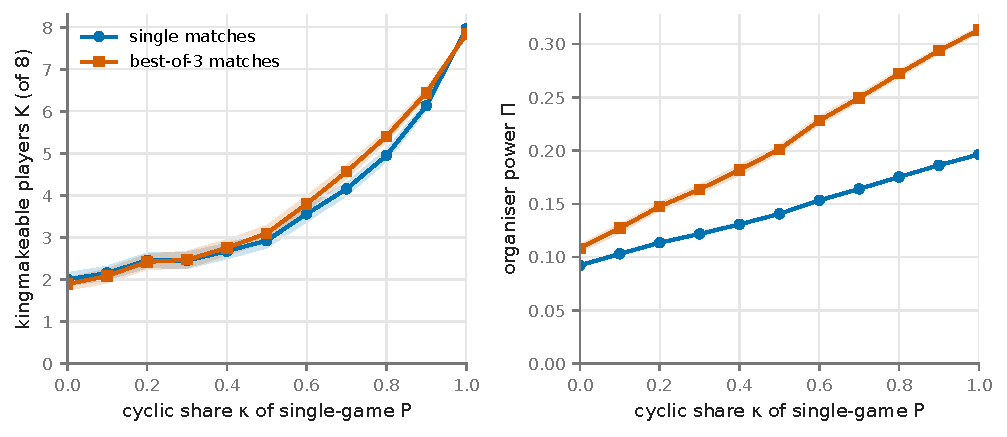
\includegraphics[width=\textwidth]{F6_bo3.pdf}
\caption{Single matches versus best-of-3 series, on the same tables (8 players, medium scale, random-skew cycles).}
\label{fig:bo3}
\end{figure}

\textbf{Best-of-3 makes the organiser more powerful, and much more so under cycles.} The average swing rises by only 1.6
points in a ladder ($+0.016$ [0.014, 0.018] at $\kap=0$) but by 11.7 points in pure rock--paper--scissors ($0.196\to0.313$ at
$\kap=1$). At $\kap=0.9$ the weakest player becomes crownable in 30\% of tables instead of 16\%. This is the
``two ingredients'' effect from Section~\ref{sec:e1}: removing luck removes the noise that protected players from bad matchups,
so who meets whom decides more. ``More games to reduce luck'' is not automatically fairer.

% ============================================================================================================
\section{Conclusion}
\label{sec:conclusion}
We asked how much of who wins a tournament is decided by the tournament when matchups are cyclic. Under a Bradley--Terry ladder,
an organiser can already choose among the top players but can never crown the weakest, a guarantee that goes back to Chung and
Hwang. As the cyclic share grows, that guarantee breaks: more players become crownable, the swing in title chances grows, and
the bottom player becomes crownable once cycles dominate, especially when matches are decisive. Whether anyone \emph{notices}
depends on the model: Bradley--Terry hides most of this power, Blade--Chest recovers it, and held-out data tell the two apart. Formats
help in a ladder world and stop helping in a cyclic one. Our main message for anyone who uses pairwise models to make decisions,
whether seeding a bracket or ranking chatbots from human votes, is that the cyclic share is worth measuring, out of sample,
before trusting a ranking.

\paragraph{Use of AI tools.} We used an AI coding assistant (Claude) to help write simulation code, run counterexample searches,
and draft parts of the text. We checked every result ourselves against the logged CSVs and exact examples, and the questions,
choices and conclusions are ours.

\bibliographystyle{plainnat}
\bibliography{refs}

% ============================================================================================================
\appendix
\section{Sanity checks}
\label{app:sanity}
All of the following pass (\texttt{outputs/csv/e0.csv}).
\begin{itemize}
\item Bracket counts: 3 and 315 canonical brackets for $n=4,8$; enumerating all $n!$ seedings gives exactly these classes.
\item Hodge split: $|\langle T,C\rangle_F|/\|L\|^2\le10^{-16}$; generated $\kap$ matches its target to $4\times10^{-16}$.
\item Dynamic program versus $10^5$ simulated tournaments: largest difference 2.4 standard errors (limit 4); versus exact
rational arithmetic at $n=4$: $10^{-16}$.
\item Limits: with very decisive ladder matches, round robin picks the top player with probability 1; with coin-flip matches
every format's winner is uniform ($\chi^2$ tests pass).
\item Nash solver: rock--paper--scissors gives $(\frac13,\frac13,\frac13)$; a BT table gives the top player.
\end{itemize}

\section{Structured cycles}
\label{app:bc2}
\begin{figure}[!htbp]
\centering
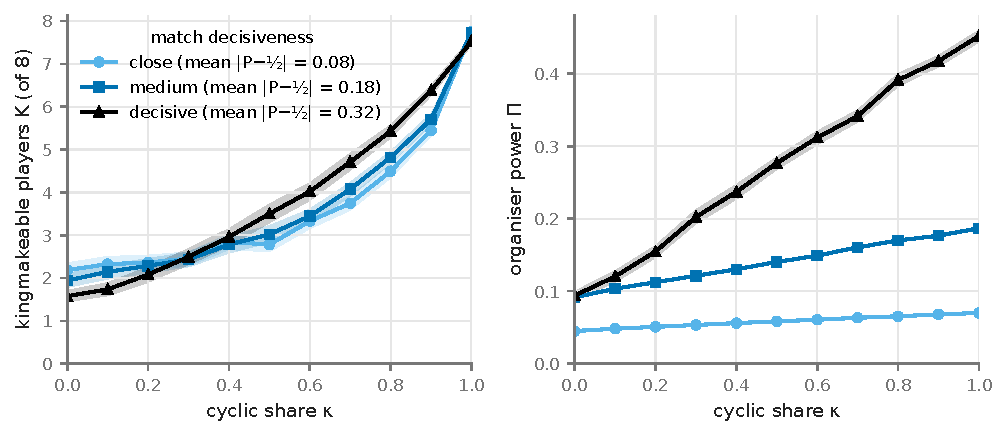
\includegraphics[width=\textwidth]{F2_power_vs_kappa_bc2.pdf}
\caption{As Figure~\ref{fig:e1}, with cycles generated from random $d=2$ blade--chest vectors (BC-d2) instead of random
skew-symmetric matrices. The trends are the same; $\Pi$ is slightly lower at high $\kap$ (decisive, $\kap=1$: 0.452 versus 0.490).}
\end{figure}

\end{document}
